\documentclass[12pt]{article}
\usepackage[top=1in,left=1in, right = 1in, footskip=1in]{geometry}
\usepackage{url}
\usepackage{graphicx}
%\usepackage{adjustbox}

\usepackage{xcolor}
\usepackage{lineno}\renewcommand\thelinenumber{\color{gray}\arabic{linenumber}}
% \linenumbers

\newcommand{\req}[1]{(\ref{#1})}

\newcommand{\eref}[1]{Eq.~\ref{eq:#1}}
\newcommand{\fref}[1]{Fig.~\ref{fig:#1}}
\newcommand{\Fref}[1]{Fig.~\ref{fig:#1}}
\newcommand{\sref}[1]{Sec.~\ref{#1}}
\newcommand{\frange}[2]{Fig.~\ref{fig:#1}--\ref{fig:#2}}
\newcommand{\tref}[1]{Table~\ref{tab:#1}}
\newcommand{\tlab}[1]{\label{tab:#1}}
\newcommand{\seminar}{SE\mbox{$^m$}I\mbox{$^n$}R}

\usepackage{amsthm}
\usepackage{amsmath}
\usepackage{amssymb}
\usepackage{amsfonts}

%\usepackage{lineno}
%\linenumbers

\usepackage[pdfencoding=auto, psdextra]{hyperref}

\usepackage[superscript,biblabel]{cite}

\bibliographystyle{vancouver}
\date{\today}

\usepackage{xspace}
\newcommand*{\ie}{i.e.\@\xspace}

\usepackage{color}

\usepackage{xspace}
\newcommand{\Rx}[1]{\ensuremath{{\mathcal R}_{#1}}\xspace}
% https://tex.stackexchange.com/questions/86565/drawbacks-of-xspace
% avoid double-\xspace
\newcommand{\Ro}{\ensuremath{{\mathcal R}_{0}}\xspace}
\newcommand{\RR}{\ensuremath{{\mathcal R}}}
\newcommand{\Rhat}{\ensuremath{{\hat\RR}}}
\newcommand{\tsub}[2]{#1_{{\textrm{\tiny #2}}}}

\newcommand{\comment}[3]{\textcolor{#1}{\textbf{[#2: }\textsl{#3}\textbf{]}}}

%% \newcommand{\rev}[1]{\comment{red}{REV}{#1}}
\newcommand{\rev}[1]{}

\newcommand{\swp}[1]{\comment{magenta}{SWP}{#1}}
\newcommand{\jd}[1]{\comment{magenta}{JD}{#1}}
\newcommand{\djde}[1]{\comment{magenta}{DJDE}{#1}}
\newcommand{\bmb}[1]{\comment{magenta}{BMB}{#1}}
\newcommand{\dc}[1]{\comment{magenta}{DC}{#1}}
\newcommand{\jsw}[1]{\comment{magenta}{JSW}{#1}}
\newcommand{\mli}[1]{\comment{magenta}{MLi}{#1}}
\newcommand{\new}[1]{\textcolor{blue}{#1}}

\begin{document}

\begin{flushleft}{
	\Large
	\textbf\newline{
		The time scale of asymptomatic transmission affects estimates of epidemic potential in the COVID-19 outbreak
	}
}
\newline
\\
Sang Woo Park B.Sc.\textsuperscript{1}
Daniel M. Cornforth Ph.D.\textsuperscript{2}
Jonathan Dushoff Ph.D.\textsuperscript{3,4,5,*}
Joshua S.\ Weitz Ph.D.\textsuperscript{2,6,*}
\\
\bigskip
\textbf{1} Department of Ecology and Evolutionary Biology, Princeton University, Princeton, NJ, USA
\\
\textbf{2} School of Biological Sciences, Georgia Institute of Technology, Atlanta, GA, USA
\\
\textbf{3} Department of Biology, McMaster University, Hamilton, Ontario, Canada
\\
\textbf{4} Department of Mathematics and Statistics, McMaster University, Hamilton, Ontario, Canada
\\
\textbf{5} M.\,G.\,DeGroote Institute for Infectious Disease Research, McMaster University, Hamilton, Ontario, Canada
\\
\textbf{6} School of Biological Sciences, Georgia Institute of Technology, Atlanta, GA, USA
\\
\textbf{7} School of Physics, Georgia Institute of Technology, Atlanta, GA, USA
\\
\bigskip

*Corresponding authors:\\
Jonathan Dushoff\\
https://mac-theobio.github.io/dushoff.html\\
dushoff@mcmaster.ca
\newline\newline
Joshua S.\ Weitz\\
http://ecotheory.biology.gatech.edu\\
jsweitz@gatech.edu\\

\end{flushleft}

\pagebreak

\section*{Abstract}

\subsection*{Background}

The role of asymptomatic carriers to transmit virus poses challenges for control of the COVID-19 pandemic. 
Study of asymptomatic transmission and implications for surveillance and disease burden is ongoing. 
There has been little study of the implications of asymptomatic transmission on dynamics of disease.

\subsection*{Methods}

We use a mathematical framework to evaluate expected effects of asymptomatic transmission on the basic reproduction number ${\cal{R}}_0$ (i.e., the expected number of secondary cases generated by an average primary case in a fully susceptible population) and the fraction of new secondary cases attributable to asymptomatic individuals.

\subsection*{Findings}

If the generation-interval distribution of asymptomatic transmission differs from that of symptomatic transmission, then estimates of the basic reproduction number which do not explicitly account for asymptomatic cases may be systematically biased. 
Specifically, if asymptomatic cases have a shorter generation interval than symptomatic cases, ${\cal{R}}_0$ will be over-estimated, and if they have a longer generation interval, ${\cal{R}}_0$ will be under-estimated.
Estimates of the realized proportion of asymptomatic transmission during the exponential phase also depend on asymptomatic generation intervals.

\subsection*{Interpretation}

Our analysis shows that understanding the temporal course of asymptomatic transmission can be important for assessing the importance of this route of transmission, and for disease dynamics. This provides an additional motivation for investigating both the prevalence and relative duration of asymptomatic transmission. 

\subsection*{Funding}

This work was supported, in part, by support from the Army Research Office to JSW (W911NF1910384), and support from the Canadian Institutes of Health Research to JD.

\pagebreak

\section*{Research in context}

\subsection*{Evidence before this study}

We searched PubMed for articles published up to March 15, 2020 using terms ``2019-nCoV'', ``novel coronavirus'', ``COVID-19'', ``SARS-CoV-2'' AND ``asymptomatic''. We found several studies describing asymptomatic infection and one study suggesting transmission by an asymptomatic carrier. 
We found one study, published on March 16, 2020, estimating the transmission rate of asymptomatic carriers of COVID-19, their prevalence, and the proportion of secondary cases caused by them.
However, we found no studies describing the effect of asymptomatic transmission in estimating the basic reproduction number of COVID-19.
To our knowledge, this is the first study to describe the effects of differences in time scales of asymptomatic and symptomatic transmission on disease dynamics.

\subsection*{Added value of this study}

We use a mathematical model to assess how the time scale of asymptomatic transmission affects the epidemic potential for COVID-like pathogens.
We compare the basic reproduction number and the proportion of secondary cases caused by asymptomatic individuals during the initial exponential growth period across a wide range of assumptions about asymptomatic transmission.
These assumptions broadly fall under two opposite scenarios: asymptomatic individuals can have fast clearance (and therefore, faster transmission) or persistent infection (and therefore, slower transmission).
If asymptomatic transmission is slower than symptomatic transmission, the basic reproduction number can be underestimated if asymptomatic transmission is not explicitly taken into account.
If asymptomatic transmission is faster than symptomatic transmission, asymptomatic transmission may still account for a large fraction of secondary infection.

\subsection*{Implications of all the available evidence}

The prevalence of asymptomatic carriers of COVID-19 and their transmission potential remain unclear. 
Future research should prioritize characterizing the course of infection for asymptomatic cases and estimating their prevalence.
%% Current estimates that do not account for asymptomatic transmission may be systematically biased and should be refined accordingly.

\pagebreak

\section{Introduction}

In an epidemic, symptomatic cases are the predominant focus of treatment and usually represent the bulk of reported cases. 
However, infected individuals who are asymptomatic yet infectious can be a critical factor in the spread of some pathogens \cite{fraser2004factors}.
Asymptomatic individuals are hard to trace, unlikely to self-isolate, and are likely to retain normal social and travel patterns \cite{quilty2020effectiveness}.

There is significant ongoing interest in asymptomatic infections in COVID-19 \cite{chan2020familial, pan2020asymptomatic, tangearly} and their transmission potential \cite{bai2020presumed} for two major reasons.
First, the proportion of infections that are asymptomatic (see~Mizumoto \textit{et al.}\cite{mizumoto_2020}) is critical to attempts to estimate the likely burden of severe outcomes (including mortality \cite{fauci_nejm2020}) when the virus spreads through a population.
Second, understanding the possible role of \emph{transmission} by asymptomatic individuals is crucial to planning surveillance and control efforts \cite{fraser2004factors}.
Given that 86\% of the cases were undocumented (i.e., mildly symptomatic or asymptomatic) in Wuhan prior to travel restrictions and may account for 79\% of infection of severe, symptomatic cases \cite{Lieabb3221}, asymptomatic cases are also likely to play an important role in the transmission of COVID-19.

Here, we focus on a third effect. 
If asymptomatic cases are important for transmission, they also have the potential to affect estimates of key parameters of disease spread such as the basic reproduction number ${\cal{R}}_0$ (i.e., the expected number of secondary cases generated by an average primary case in a fully susceptible population \cite{anderson1992infectious}). 
Thus, we investigate the relationship between individual-level features of asymptomatic cases (e.g., the probability that an infection is asymptomatic, asymptomatic case duration, transmission by asymptomatic individuals) to dynamics at the population scale.

\section{Methods}

We model viral spread using a renewal-equation framework \cite{heesterbeek1996concept}, which allows us to model the current incidence of infected individuals (i.e., the rate at which new infections occur in the population) as a function of previous incidence and how infectiousness of an infected individual varies over the course of their infection.
We divide incidence $i$ into two categories -- $i_a$ and $i_s$ -- corresponding to incidence of asymptomatic and symptomatic cases, respectively.
Newly infected individuals that are either asymptomatically or symptomatically infected can transmit the disease to others, but they differ in their intrinsic reproduction numbers, ${\cal{R}}_a$ and ${\cal{R}}_s$, respectively, as well as intrinsic generation-interval distributions \cite{champredon2015intrinsic}, $g_a(\tau)$ and $g_s(\tau)$.
Generation intervals, which are defined as the time between when an individual is infected and when that individual infects another person \cite{svensson2007note}, depend on the natural history of infection:
individuals with subclinical infections may have fast clearance and short generation intervals, or persistent infection and long generation intervals (cf. Roberts and Heesterbeek\cite{roberts2007model}).
The shape of the generation-interval distribution characterizes the relationship between the epidemic growth rate $r$ and the reproduction number \cite{wallinga2007generation}.

Neglecting births and loss of immunity on the time scale of the outbreak, the dynamics of susceptibles and incidence are:
\begin{eqnarray}
\dot{S}&=&-i(t) \\
i(t)&=&\mathcal R_a S(t) \int_0^\infty i_a(t-\tau) g_a(\tau) \mathrm{d}\tau + \mathcal R_s S(t) \int_0^\infty i_s(t-\tau) g_s(\tau) \mathrm{d}\tau.
\end{eqnarray}
The basic reproduction number of this system is:
\begin{equation}
{\cal{R}}_{0}= p {\cal{R}}_a + (1-p) {\cal{R}}_s,
\end{equation}
where $p$ is the proportion of \emph{incident cases} that are asymptomatic: $i_a(t) = p i(t)$.
The corresponding intrinsic generation-interval distribution of an average infected individual is given by: 
\begin{equation}
g(\tau) = z g_a(\tau) + (1-z) g_s(\tau),
\end{equation}
where we define the ``intrinsic'' proportion of asymptomatic transmission $z$ as the relative contribution of asymptomatic cases to the basic reproduction number:
\begin{equation}
z = p {\cal{R}}_a/{\cal{R}}_{0}.
\end{equation}
Note that the intrinsic proportion of symptomatic transmission satisfies
\begin{equation}
1-z = (1-p) {\cal{R}}_s/{\cal{R}}_{0}.
\end{equation}
Yet, this information is not sufficient to disentangle the role of asymptomatic cases, i.e., what fraction of secondary cases can be ascribed to \emph{realized} transmission from asymptomatic cases vs.~symptomatic cases?

The intrinsic proportion of asymptomatic transmission $z$ is a useful benchmark, but does not necessarily reflect the realized proportion of asymptomatic transmission, unless both types of infection have the same generation-interval distribution.
The \emph{realized} proportion of asymptomatic transmission, $q$ at time $t$ is given by:
\begin{equation}
\frac{q}{1-q}=\frac{\mathcal R_a S(t) \int_0^\infty i_a(t-\tau) g_a(\tau) \mathrm{d}\tau}{\mathcal R_s S(t) \int_0^\infty i_s(t-\tau) g_s(\tau) \mathrm{d}\tau}.
\end{equation}
During the period of exponential growth, we assume $S$ remains nearly constant, and $i(t)$ is proportional to $\exp(r t)$, and simplify by recalling that $i_a(t)= p i(t)$, $i_s(t)=(1-p)i(t)$ such that: 
\begin{equation}
\frac{q}{1-q}=\left(\frac{z}{1-z}\right)\frac{\delta_a}{\delta_s}.
\label{eq.qratio}
\end{equation}
Here, $\delta_c$ for each of the two classes is the average ``discount'' of a new infection -- the average relative contribution of a secondary infection to the epidemic, taking exponential growth into account:
\begin{equation}
	\delta_c = \int_0^\infty \exp(-r\tau) g_c(\tau) \mathrm{d}\tau.
\end{equation}
$\delta_c<1$ and grows smaller as the generation interval grows longer.
Thus, the realized proportion of asymptomatic infections will be increased (resp., decreased) if transmission is relatively faster (slower) along the asymptomatic route.
The discount $\delta$ also depends on the relative variation in the generation-interval distribution, the ``dispersion'': more variation in generation intervals leads to more opportunities for fast spread and thus to higher values of $\delta$ (similar to shorter average generation intervals). 

To estimate the effects of assumptions about asymptomatic transmission on the importance of asymptomatic transmission and estimates of the basic reproduction number ${\cal{R}}_0$, we parameterize the generation interval distributions of asymptomatic and symptomatic cases based on their means, $\bar G_a$ and $\bar G_s$, and dispersions, $\kappa_a$ and $\kappa_s$.
We assume that generation intervals are gamma distributed, and we set the dispersion to be equal to the squared coefficient of variation (the reciprocal of the gamma shape parameter, see Supplementary Materials).
We assume that epidemic growth rate $r$ and the generation-interval distribution of symptomatic case are known, using parameter values that are consistent with earlier COVID-19 models \cite{park_preprint}: $1/r=7$ days, $\bar G_s=8$ days, and $\kappa_s=0.5$.
We infer values of $q$ using Eq.~\req{eq.qratio} and ${\cal{R}}_0$ using the Euler-Lotka equation \cite{lotka1907relation}:
\begin{equation}
\frac{1}{\mathcal R_0} = \int \exp(-r \tau) g(\tau) \mathrm{d} \tau.
\end{equation}
In Supplementary Materials, we also use an ordinary differential equation model including both asymptomatic and symptomatic cases to give a concrete example of how differences in generation intervals affect both $q$ and estimates of $\mathcal R_0$.

\section{Results}

\begin{figure*}[b!]
\begin{center}
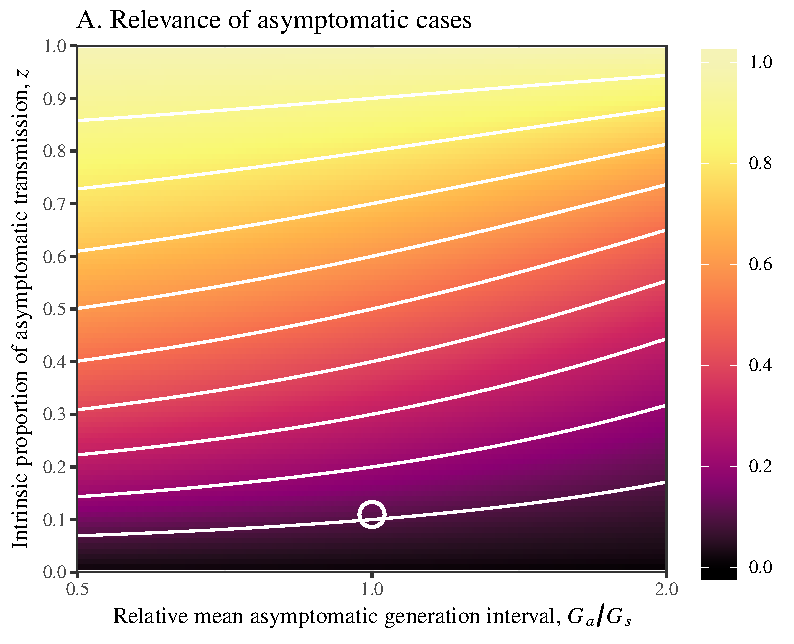
\includegraphics[width=0.45\textwidth]{../figheatmap.pdf}
\mbox{\hspace{0.05\textwidth}}
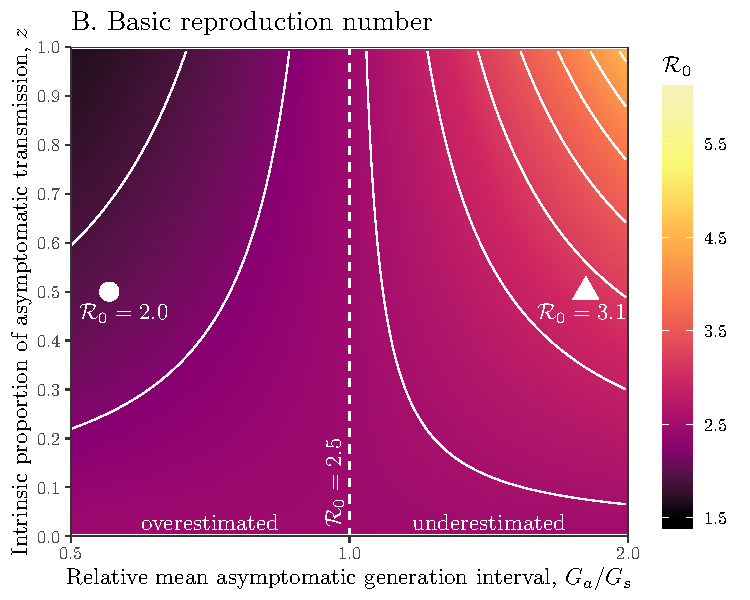
\includegraphics[width=0.45\textwidth]{../figheatmap_R0.pdf}
\caption{Effects of intrinsic proportion of asymptomatic transmission on the realized proportion of asymptomatic transmission and basic reproduction number, given variation in
the mean generation interval of asymptomatic cases. 
(A) Increasing the speed of asymptomatic transmission (shorter generation intervals) increases the realized proportion of asymptomatic transmission, $q$.
(B) Increasing the speed of asymptomatic transmission (shorter generation intervals) decreases the basic reproduction number ${\cal{R}}_0$.
When $\bar G_a$ is smaller (larger) than $\bar G_s$, estimates based on the observed generation distribution for symptomatic cases (${\cal{R}}_0=2.5$; dashed line) are expected to over- (under-) estimate the true $\mathcal R_0$.
Triangle denotes $z=0.5$ and $\bar G_a/\bar G_s = 0.55$.
Circle denotes $z=0.5$ and $\bar G_a/\bar G_s = 1.8$.
Solid lines show contours for $q$ and \Ro\ values. 
Here, we assume $1/r=7$ days, $\bar G_s=8$ days, and $\kappa_s=\kappa_a=0.5$.
\label{fig.importance}}
\end{center}
\end{figure*}

We explore the effects of different assumptions about speed and effectiveness of asymptomatic transmission on the importance of asymptomatic transmission and estimates of the basic reproduction number ${\cal{R}}_0$, using a gamma assumption (see Methods).
Across the range of parameters we explore, the intrinsic proportion of asymptomatic transmission $z$ is similar to the realized proportion $q$ (Figure~\ref{fig.importance}A).
As the relative mean generation interval of asymptomatic transmission, $\bar G_a/\bar G_s$, increases, $q$ decreases because symptomatic cases are more likely to have short generation intervals (i.e., fast transmission events), which drive the spread during the growth phase (Figure~\ref{fig.importance}A).

Figure~\ref{fig.importance}B shows the effect of different assumptions about the generation interval of asymptomatic cases, $\bar G_a$, on the basic reproduction number ${\cal{R}}_0$.
When $\bar G_a$ is long compared to $\bar G_s$, then we are effectively assuming a longer mean for the overall generation interval. 
This assumption leads to a larger estimate of \Ro\ for a fixed value of $r$ (see~Park \textit{et al.}\cite{park_2019practical}).
Conversely, when $\bar G_a < \bar G_s$, generation intervals are shorter, leading to lower estimates of the epidemic strength \Ro. Both of these effects are stronger when the intrinsic proportion of asymptomatic transmission $z$ increases (and disappear as $z\to0$).
Therefore, when ${\cal{R}}_0$ is estimated without explicitly accounting for asymptomatic spread (white, dashed line in Figure~\ref{fig.importance}B), it can be over- or under- estimated depending on the relative duration of infection between symptomatic and asymptomatic individuals.
The qualitative effects of $z$ and $\bar G_a/\bar G_s$ on $q$ and ${\cal{R}}_0$ remain robust when we assume narrower ($\kappa_s = \kappa_a = 0.3$; Figure~S1) or wider ($\kappa_s = \kappa_a = 0.8$; Figure~S2) generation intervals.

Relative generation-interval dispersion of asymptomatic cases $\kappa_a/\kappa_s$ have similar, but smaller, effects on $q$ and ${\cal{R}}_0$ (Figure~S3).
Since a wider generation-interval distribution has a higher proportion of early transmission than a narrow one, increasing the generation-interval dispersion has qualitatively similar effects on $q$ and ${\cal{R}}_0$ as decreasing the mean generation interval.

\section{Discussion}

Much is still unknown about the time scale and effectiveness of asymptomatic transmission in COVID-19.
Here we highlight the need to characterize the generation-interval distribution for asymptomatic transmission, and its consequences not only for contact tracing but for estimation of the basic reproduction number of the ongoing COVID-19 outbreak~\cite{park_preprint} and of the effective proportion of asymptomatic transmission during the exponential-growth phase.
Our reproductive number findings fit into a broader framework linking epidemic speed, strength, and generation intervals -- for a given observed speed increases in the mean generation interval imply larger reproduction number~\cite{wearing2005appropriate, roberts2007model, wallinga2007generation, powers2014impact, park_2019practical}.

If asymptomatic infections are more persistent than symptomatic ones, the mean generation interval for COVID-19 could be longer than estimated from symptomatic cases alone -- possibly increasing ${\cal{R}}_0$ (Figure~\ref{fig.importance}B).
However, if asymptomatic cases tend to resolve quickly, then current estimates of ${\cal{R}}_0$ may be over-estimates of the underlying strength (Figure~\ref{fig.importance}B), and asymptomatic cases may be driving a larger fraction of secondary cases than we would expect without accounting for their differences (Figure~\ref{fig.importance}A).
Note that cases do not have to be completely asymptomatic for our qualitative results to apply.
People with mild symptoms unlikely to be diagnosed in a particular time and place (sometimes referred to as subclinical cases) are expected to affect transmission patterns in the same way.

We focus here on the exponential phase, so it is worth noting that the realized proportion of asymptomatic transmission $q$ is time-dependent, varying with dynamic changes in incidence and proportion susceptible. 
Future work might also consider the ways in which asymptomatic individuals can modulate the catalysis of epidemics in a networked metapopulation~\cite{watts_pnas2005, chinazzi2020effect, du2020risk}.
Characterizing the role of asymptomatic individuals in driving the persistence of the epidemic will be critical for assessing the post-pandemic outcome \cite{lipsitch_preprint}.

\mbox{}\\
\noindent
\textbf{Acknowledgments:} The authors thank John Glasser for comments
and discussion on the manuscript, particularly on short notice. 
\newline\newline
\noindent
\textbf{Data Availabililty:} All code is available at\\
https://github.com/mac-theobio/coronavirus\_asymptomatic.
\newline\newline
\noindent
\textbf{Competing interests:} We declare no competing interests.

\pagebreak

\section*{Supplementary Materials}
\renewcommand\thefigure{S\arabic{figure}}
\renewcommand\theequation{S\arabic{equation}}
\setcounter{figure}{0}
\setcounter{equation}{0}

\subsection*{A gamma approximation to generation-interval distributions}

Assuming that the intrinsic generation-interval distribution for each class (asymptomatic and symptomatic) follows a gamma distribution with mean $\bar G_c$ and dispersion $\kappa_c$, the average discount of a new infection can be written as:
\begin{equation}
\delta_c = (1 + \kappa_c r \bar G_c)^{-1/\kappa_c},
\end{equation}
which shows that the average discount increases with smaller $\bar G_c$ and with larger $\kappa_c$.
Then, the odds of the realized proportion of asymptomatic transmission can be written as:
\begin{equation}
\frac{q}{1-q}=\left(\frac{z}{1-z}\right)\left[\frac{(1 + \kappa_a r \bar G_a)^{-1/\kappa_a}}{(1 + \kappa_s r \bar G_s)^{-1/\kappa_s}}\right],
\end{equation}
where $\bar G_a$ and $\bar G_s$ are the mean generation intervals for asymptomatic and symptomatic cases, and $\kappa_a$ and $\kappa_s$ are the generation-interval dispersions for asymptomatic and symptomatic cases.
Finally, the basic reproduction number is calculated by using the Euler-Lotka equation:
\begin{equation}
\mathcal R_0 = \left(z (1 + \kappa_a r \bar G_a)^{-1/\kappa_a} + (1-z) (1 + \kappa_s r \bar G_s)^{-1/\kappa_s}\right)^{-1}.
\end{equation}

\subsection*{A compartmental model for asymptomatic/symptomatic cases}

Consider an SEIR model variant in which an infected individual can be either asymptomatic, $I_a$, or symptomatic, $I_s$.
We note that $I_a$ and $I_s$ represent prevalence (i.e., the total number of currently infectious individuals) of asymptomatic and symptomatic individuals; these quantities are different from $i_s$ and $i_s$ that we present in the main text, which represent incidence (i.e., the rate at which new cases are generated)  of asymptomatic and symptomatic individuals.
While both cases can recover, we assume that only symptomatic cases can lead to fatalities, denoted
by the $D$ category.
In total, the dynamics of susceptibles, exposed, infectious, recovered, and dead are:
\begin{eqnarray}
\dot{S}&=&-\beta_a S I_a -\beta_s S I_s \\
\dot{E}&=&\beta_a S I_a +\beta_s S I_s -\gamma_e E\\
\dot{I}_a&=&p\gamma_e E-\gamma_a I_a\\
\dot{I}_s&=&(1-p)\gamma_e E-\gamma_s I_s\\
\dot{R}&=&\gamma_a I_a + (1-f)\gamma_s I_s \\
\dot{D}&=&f\gamma_s I_s.
\end{eqnarray}
Here, $\beta_a$ and $\beta_s$ denote transmission rates,
$\gamma_e$ denotes the transition from exposed to infectious,
$p$ is the fraction of asymptomatic cases that
are generated for each exposed individual,
$1-p$ is the fraction of symptomatic cases that
are generated for each exposed individual,
$\gamma_a$ and $\gamma_s$ denote recovery rates,
and $f$ denotes the case fatality ratio for symptomatic cases.

Given that the number of infected individuals increase exponentially at rate $r$ initially, the equations
for the infectious cases can be rewritten given the ansatz
$E(t)=c_e e^{rt}$,
$I_a(t)=c_a e^{rt}$,
$I_s(t)=c_s e^{rt}$.
Then, it follows that 
\begin{eqnarray}
r c_a&=&p\gamma_e c_e-\gamma_a c_a,\\
r c_s&=&(1-p)\gamma_e c_e-\gamma_s c_s,
\end{eqnarray} 
which implies that
\begin{equation}
\frac{c_a}{c_s}=\frac{p}{1-p}\left[\frac{r+\gamma_s}{r+\gamma_a}\right].
\end{equation}
This shows that the prevalence of asymptomatic and symptomatic individuals is different from $p$ and $1-p$ because prevalence measures the individuals that are currently infectious and does not account for individuals that have already recovered.
Finally, the ratio of secondary case production caused by asymptomatic vs.~symptomatic
individuals during the exponential phase should be
\begin{equation}
\frac{q}{1-q} = \left(\frac{\beta_a}{\beta_s}\right)\frac{p}{1-p}\left[\frac{r+\gamma_s}{r+\gamma_a}\right],
\end{equation}
where $q$ is the fraction of new secondary cases caused by
asymptomatic individuals.

The basic reproduction number of this system is:
\begin{equation}
{\cal{R}}_{0}= p {\cal{R}}_a + (1-p) {\cal{R}}_s,
\end{equation}
where 
\begin{eqnarray}
{\cal{R}}_a &=& \frac{\beta_a}{\gamma_a},\\
{\cal{R}}_s &=& \frac{\beta_s}{\gamma_s}.
\end{eqnarray}
The generation-interval distributions for asymptomatic and symptomatic individuals follow the same functional form as the corresponding generation-interval distribution for a single-type SEIR model since both asymptomatic and symptomatic individuals have exponentially distributed latent and infectious periods \cite{svensson2015influence}:
\begin{eqnarray}
g_a(\tau) &=& \frac{\gamma_e \gamma_a}{\gamma_e - \gamma_a} \left(\exp(-\gamma_a \tau) - \exp(-\gamma_e \tau)\right),\\
g_s(\tau) &=& \frac{\gamma_e \gamma_s}{\gamma_e - \gamma_s} \left(\exp(-\gamma_s \tau) - \exp(-\gamma_e \tau)\right).
\end{eqnarray}
It immediately follows that 
\begin{equation}
\left(\frac{z}{1-z}\right)\left[\frac{\int_0^\infty \exp(-r\tau) g_a(\tau) \mathrm{d}\tau}{\int_0^\infty \exp(-r\tau) g_s(\tau) \mathrm{d}\tau}\right] = \left(\frac{\beta_a}{\beta_s}\right)\frac{p}{1-p}\left[\frac{r+\gamma_s}{r+\gamma_a}\right],
\end{equation}
where $z = p {\cal{R}}_a/{\cal{R}}_{0}$ and $1-z=(1-p) {\cal{R}}_s/{\cal{R}}_{0}$ -- compare to Eq.~(8) in the main text.

\pagebreak

\subsection*{Supplementary figures}

\begin{figure*}[!ht]
\begin{center}
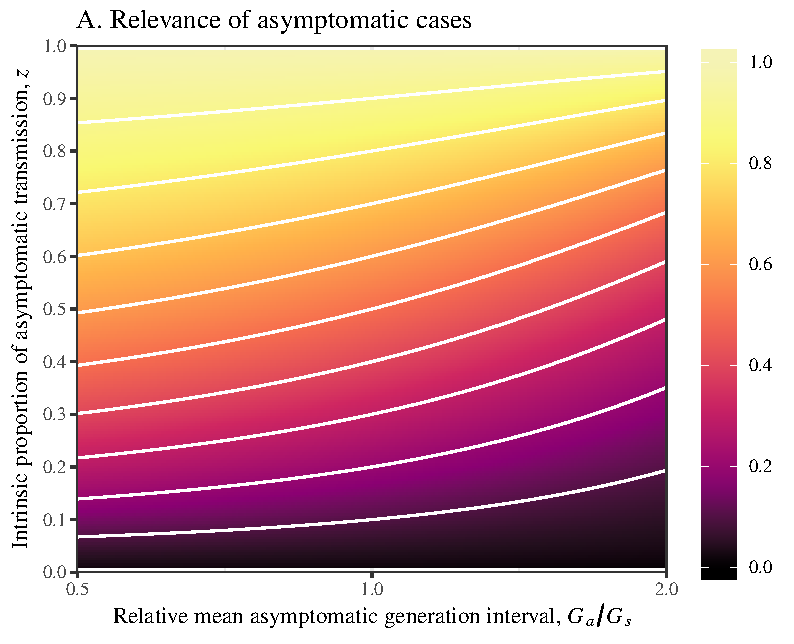
\includegraphics[width=0.45\textwidth]{../figheatmap_03.pdf}
\mbox{\hspace{0.05\textwidth}}
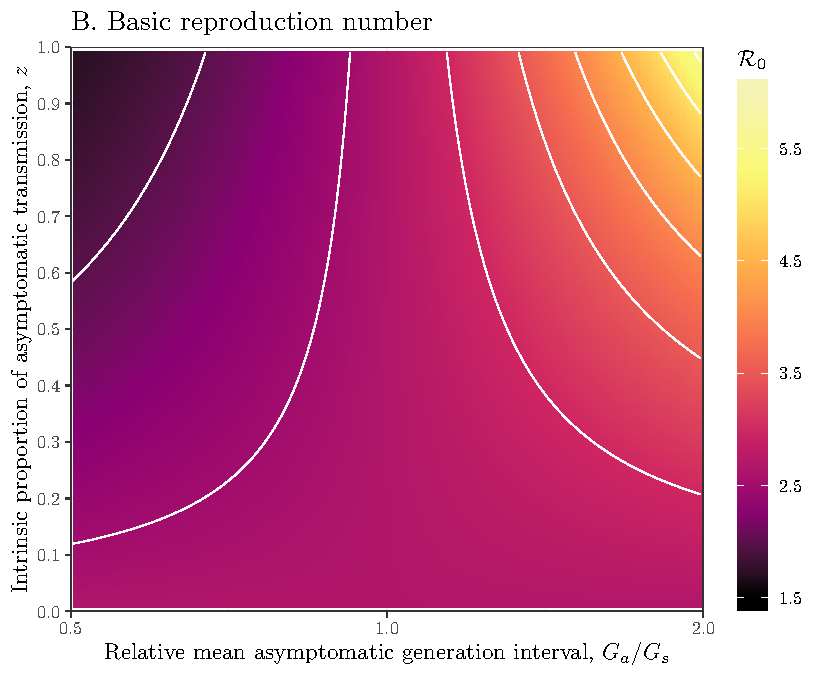
\includegraphics[width=0.45\textwidth]{../figheatmap_R0_03.pdf}
\caption{Effects of intrinsic proportion of asymptomatic transmission on the realized proportion of asymptomatic transmission and basic reproduction number, given variation in
the mean generation interval of asymptomatic cases when generation-interval distributions are narrow. 
Here, we assume $1/r=7$ days, $\bar G_s=8$ days, and $\kappa_s=\kappa_a=0.3$.
See Figure 1 in the main text for figure caption.
}
\end{center}
\end{figure*}

\pagebreak

\begin{figure*}[!ht]
\begin{center}
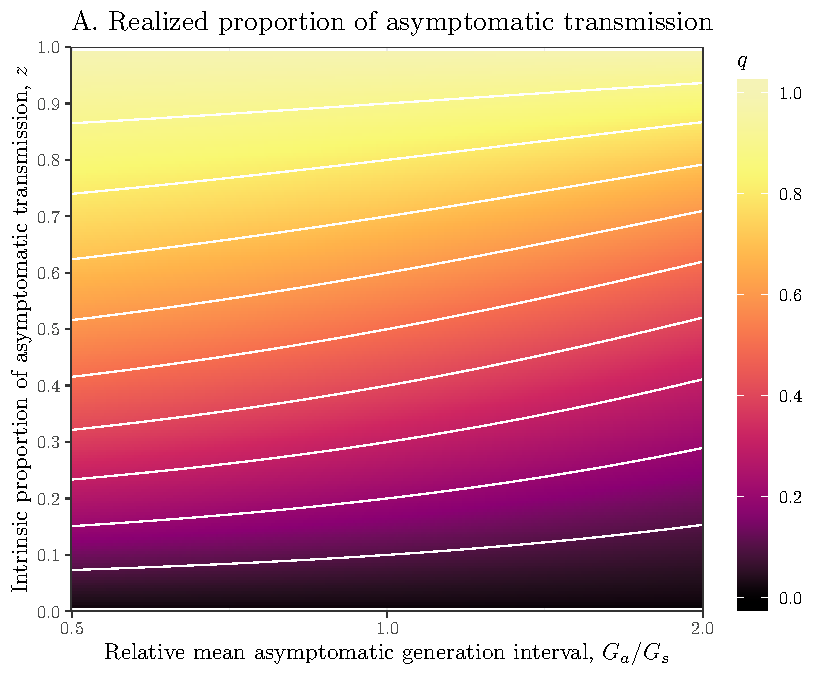
\includegraphics[width=0.45\textwidth]{../figheatmap_08.pdf}
\mbox{\hspace{0.05\textwidth}}
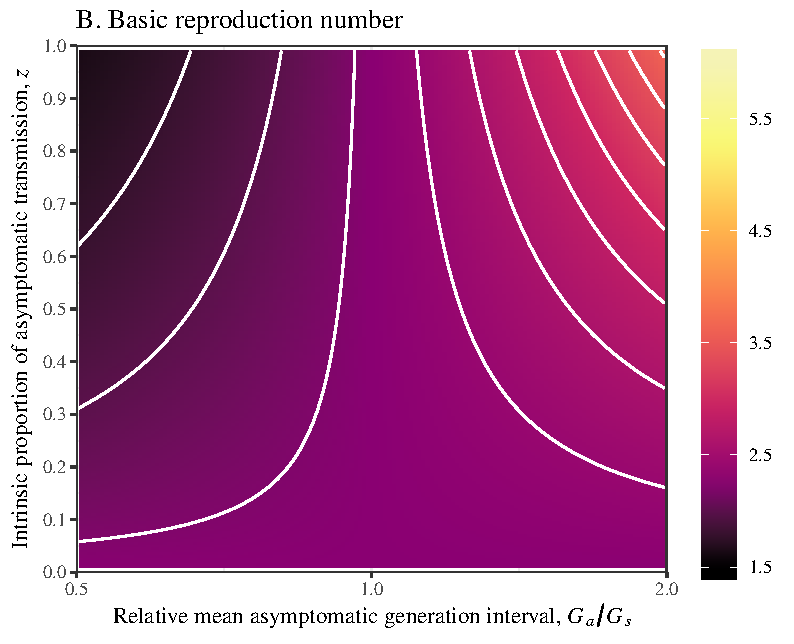
\includegraphics[width=0.45\textwidth]{../figheatmap_R0_08.pdf}
\caption{Effects of intrinsic proportion of asymptomatic transmission on the realized proportion of asymptomatic transmission and basic reproduction number, given variation in
the mean generation interval of asymptomatic cases when generation-interval distributions are wide. 
Here, we assume $1/r=7$ days, $\bar G_s=8$ days, and $\kappa_s=\kappa_a=0.8$.
See Figure 1 in the main text for figure caption.
}
\end{center}
\end{figure*}

\pagebreak

\begin{figure*}[!ht]
\begin{center}
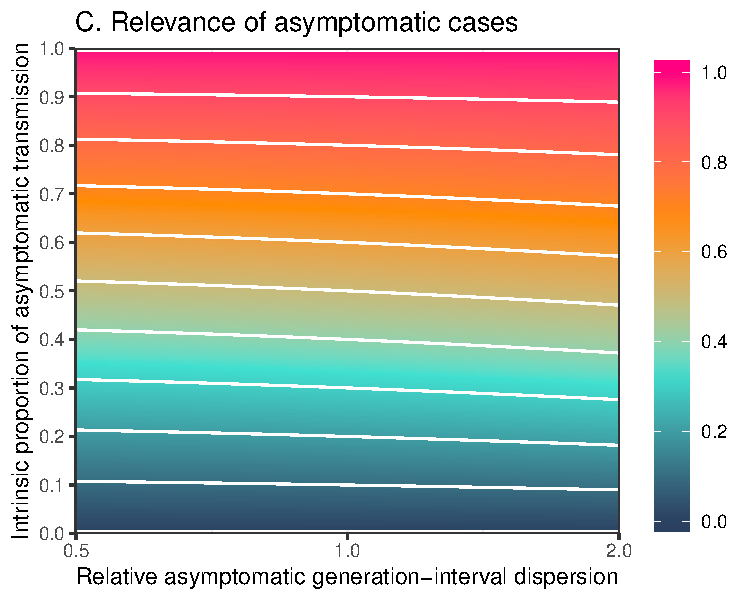
\includegraphics[width=0.45\textwidth]{../figheatmap_kappa.pdf}
\mbox{\hspace{0.05\textwidth}}
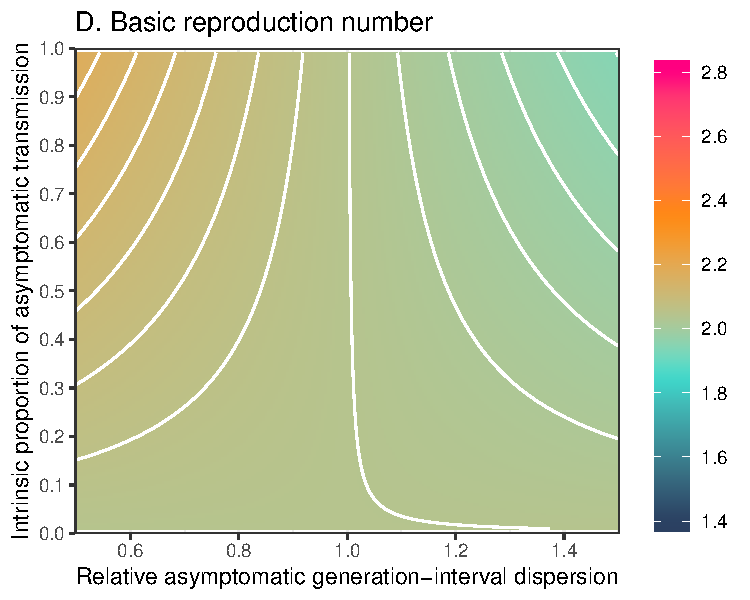
\includegraphics[width=0.45\textwidth]{../figheatmap_kappa_R0.pdf}
\caption{Effects of intrinsic proportion of asymptomatic transmission on the realized proportion of asymptomatic transmission and basic reproduction number, given variation in
the generation-interval dispersion of asymptomatic cases.
(A) Wide/narrow generation intervals of asymptomatic cases increase/decrease the relevance of asymptomatic cases, $q$.
(B) Wide/narrow generation intervals of asymptomatic cases decrease/increase the basic reproduction number ${\cal{R}}_0$.
Solid lines show contours for $q$ and \Ro\ values.
Here, we assume $1/r=7$ days, $\bar G_s=\bar G_a=8$ days, and $\kappa_s=0.5$.
}
\end{center}
\end{figure*}

\pagebreak

\bibliography{coronavirus_abbv.bib}

\end{document}
